\documentclass[11pt]{article}
\usepackage[utf8]{inputenc}
\usepackage{amsfonts, amssymb, amsmath}
\usepackage[a4paper, margin=1.1in]{geometry}
\usepackage{tikz}
\usetikzlibrary{decorations.text}
\usepackage{float}
\usepackage{wrapfig}
\usepackage{graphicx} % required for inserting images
\usepackage[margin=2cm]{caption}
\usepackage[backend=biber, sorting=none]{biblatex}
\usepackage{hyperref}
\usepackage{listings}
\usepackage{xcolor}

\definecolor{codegreen}{rgb}{0,0.6,0}
\definecolor{codegray}{rgb}{0.5,0.5,0.5}
\definecolor{codepurple}{rgb}{0.58,0,0.82}
\definecolor{backcolour}{rgb}{0.95,0.95,0.92}

\lstdefinestyle{mystyle}{
    backgroundcolor=\color{backcolour},   
    commentstyle=\color{codegreen},
    keywordstyle=\color{magenta},
    % numberstyle=\tiny\color{codegray},
    stringstyle=\color{codepurple},
    basicstyle=\ttfamily\footnotesize,
    breakatwhitespace=false,         
    breaklines=true,                 
    captionpos=b,                    
    keepspaces=true,                 
    % numbers=left,                    
    % numbersep=5pt,                  
    showspaces=false,                
    showstringspaces=false,
    showtabs=false,                  
    tabsize=2
}

\lstset{style=mystyle}
\renewcommand{\figureautorefname}{Fig.}
\renewcommand{\equationautorefname}{Eq.}
\renewcommand{\tableautorefname}{Tab.}
\renewcommand{\subsectionautorefname}{Section.}
\renewcommand{\sectionautorefname}{Section.}

\renewcommand{\arraystretch}{1.5}

\addbibresource{bibliography/sample.bib}
\def\fooA
{
    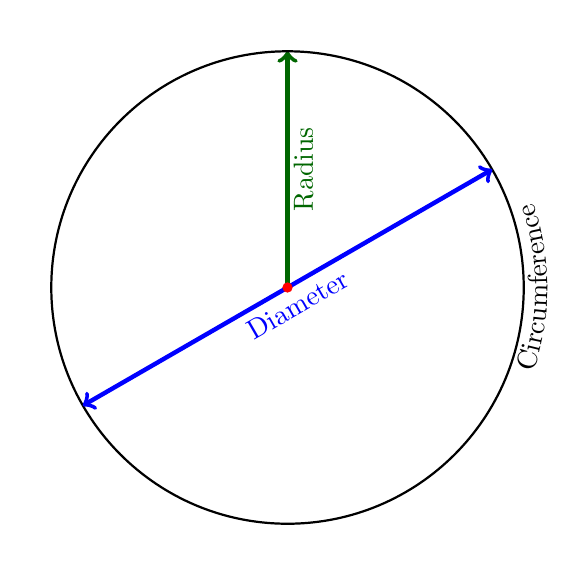
\begin{tikzpicture}
        \path[decorate,
            decoration={text along path,
                    text={Circumference},
                    text align=center}] (0,0) circle (-3.3 cm);
        \draw[ultra thick, black!60!green, ->] (0,0) -- (0,3);
        \draw (0.2,1.5) node[rotate=90, black!60!green] {Radius};
        \draw[thick] (0,0) circle (3);
        \draw[ultra thick, blue, <->] (-2.6,-1.5) -- (2.6,1.5);
        \draw[thick, fill=red, red] (0,0) circle (0.5mm) node[below, blue, rotate = 30] {Diameter};
    \end{tikzpicture}
}

\def\figRod
{
    \begin{figure}[H]
        \centering
        {
            \begin{tikzpicture}
                \draw (-3,1) -- (3,1);
                \draw (-3,-1) -- (3,-1);
                \draw (3,0) ellipse (0.2 and 1);
                \draw (-3,-1) arc (270:90:0.2 and 1);
                \draw[|->] (0,0) node[below] {$_o$} -- (1,0) node[right] {$x$};
                \draw[|-|] (-3,-1.5) -- (0,-1.5) node[below] {$2L$} -- (3,-1.5);
            \end{tikzpicture}
        }
        \caption{1D rod model for visualization (the length is only relevant in the $x$-dimension, all other dimensions should be assumed as zero) }
        \label{fig:Rod}
    \end{figure}
}

\def\figDescretizedDomain
{
    \begin{figure}[H]
        \centering
        {
            \begin{tikzpicture}
                % \draw[step=0.5cm, gray, very thin] (0,0) node[black, above=5mm] {$-L/2$} grid (8,0.5) node[black, above] {$+L/2$};
                \draw[step=0.5cm, gray, very thin] (0,0) grid (3.2,0.5);
                \draw[step=0.5cm, gray, very thin] (4.8,0) grid (8,0.5);
                \draw[|<->|] (0,-0.5) -- (8,-0.5);
                \draw[|-|] (1,0.7) -- (1.5,0.7);
                \draw[|->] (4,-0.15) node[below] {$_o$} -- (4.5,-0.15) node[right] {$x$};
                \node at (1.25,0.7) [above] {$h$};
                \node at (0,-0.5) [left] {$-L$};
                \node at (8,-0.5) [right] {$+L$};
                \node at (4,-0.5) [below] {$2L$};
                \foreach \x in {3.5,4,4.5} {
                        \foreach \y in {0.25} {
                                \fill[black] (\x, \y) circle (0.5mm);
                            }
                    }
            \end{tikzpicture}
        }
        \caption{Discretized domain of the 1D geometry from \autoref{fig:Rod}.}
        \label{fig:DescretizedDomain}
    \end{figure}
}

\def\figSolutionMat
{
    \begin{figure}[H]
        \centering
        {
            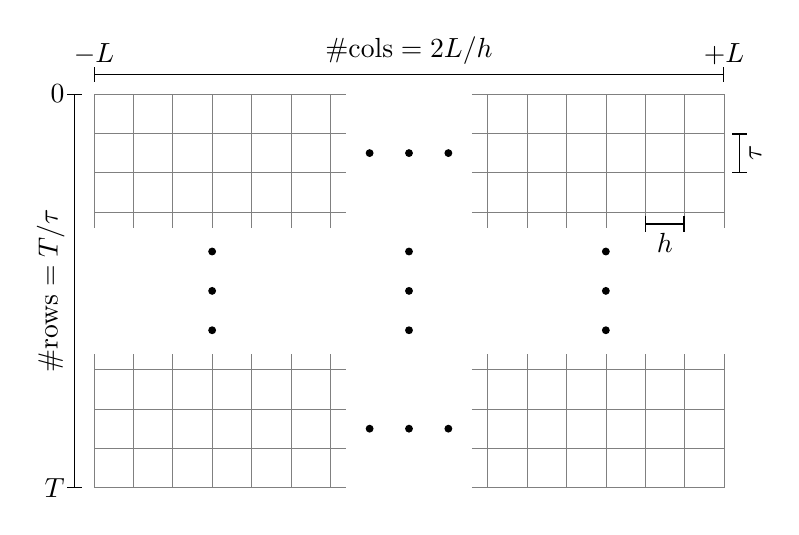
\begin{tikzpicture}
                % \draw[step=0.5cm, gray, very thin] (0,0) node[black, above=5mm] {$-L/2$} grid (8,0.5) node[black, above] {$+L/2$};
                \draw[step=0.5cm, gray, very thin] (0,0) grid (3.2,1.7);
                \draw[step=0.5cm, gray, very thin] (4.8,0) grid (8,1.7);
                \draw[step=0.5cm, gray, very thin] (0,3.3) grid (3.2,5);
                \draw[step=0.5cm, gray, very thin] (4.8,3.3) grid (8,5);
                \foreach \x in {3.5,4,4.5} {
                        \foreach \y in {0.75} {
                                \fill[black] (\x, \y) circle (0.5mm);
                            }
                    }
                \foreach \x in {1.5} {
                        \foreach \y in {2,2.5,3} {
                                \fill[black] (\x, \y) circle (0.5mm);
                            }
                    }

                \foreach \x in {4} {
                        \foreach \y in {2,2.5,3} {
                                \fill[black] (\x, \y) circle (0.5mm);
                            }
                    }

                \foreach \x in {6.5} {
                        \foreach \y in {2,2.5,3} {
                                \fill[black] (\x, \y) circle (0.5mm);
                            }
                    }

                \foreach \x in {3.5,4,4.5} {
                        \foreach \y in {4.25} {
                                \fill[black] (\x, \y) circle (0.5mm);
                            }
                    }


                \node at (4,5.25) [above] {$\text{\#cols}=2L/h$};
                \draw[|-|] (0,5.25) node[above] {$-L$} -- (8,5.25) node[above] {$+L$};

                \node at (-0.25,2.5) [above,rotate=90] {$\text{\#rows}=T/\tau$};
                \draw[|-|] (-0.25,0) node[left] {$T$} -- (-0.25,5) node[left] {$0$};

                \draw[|-|] (7,3.35) -- (7.5,3.35);
                \node at (7.25,3.35) [below] {$h$};

                \draw[|-|] (8.2,4) -- (8.2,4.5);
                \node at (8.2,4.25) [below,rotate=90] {$\tau$};

            \end{tikzpicture}
        }
        \caption{Solution Matrix. Each cell represents the value of $v$ at a particular time $\tau$ and space $h$. The boundaries are not shown as they are not part of the final solution.}
        \label{fig:SolutionMat}
    \end{figure}
}

\def\figDDecompose
{
    \begin{figure}[H]
        \centering
        {
            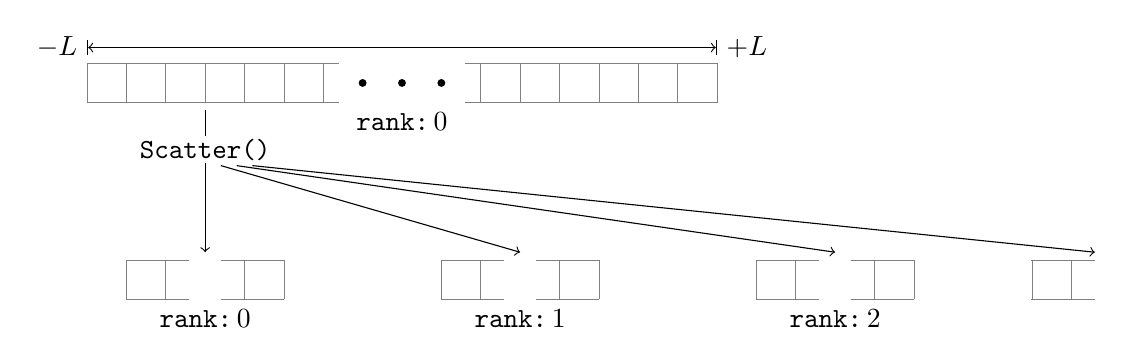
\begin{tikzpicture}
                % \draw[step=0.5cm, gray, very thin] (0,0) node[black, above=5mm] {$-L/2$} grid (8,0.5) node[black, above] {$+L/2$};
                \draw[|<->|] (-1.5,0.7) node[left] {$-L$} -- (6.5,0.7) node[right] {$+L$};
                \draw[step=0.5cm, gray, very thin] (-1.5,0) grid (1.7,0.5);
                \draw[step=0.5cm, gray, very thin] (3.3,0) grid (6.5,0.5);
                \foreach \x in {2,2.5,3} {
                        \foreach \y in {0.25} {
                                \fill[black] (\x, \y) circle (0.5mm);
                            }
                    }
                \node at (2.5,0) [below] {$\texttt{rank:}\, 0$};
                \begin{scope}[yshift=0]
                    \draw[->] (0,-0.1) -- (0,-0.6) node[fill=white, inner sep=1pt] {\texttt{Scatter()}} -- (0,-1.9);
                    \draw[->] (0.2,-0.8) -- (4,-1.9);
                    \draw[->] (0.4,-0.8) -- (8,-1.9);
                    \draw[->] (0.6,-0.8) -- (11.3,-1.9);

                    % \draw[step=0.5cm, gray, very thin] (-3.3,-2) grid (-2.5,-2.5);

                    \draw[step=0.5cm, gray, very thin] (-1,-2) grid (-0.2,-2.5);
                    \draw[step=0.5cm, gray, very thin] (0.2,-2) grid (1,-2.5);
                    \node at (0,-2.5) [below] {$\texttt{rank:}\, 0$};

                    \draw[step=0.5cm, gray, very thin] (2.99,-2) grid (3.8,-2.5);
                    \draw[step=0.5cm, gray, very thin] (4.2,-2) grid (5,-2.5);
                    \node at (4,-2.5) [below] {$\texttt{rank:}\, 1$};

                    \draw[step=0.5cm, gray, very thin] (6.99,-2) grid (7.8,-2.5);
                    \draw[step=0.5cm, gray, very thin] (8.2,-2) grid (9,-2.5);
                    \node at (8,-2.5) [below] {$\texttt{rank:}\, 2$};

                    \draw[step=0.5cm, gray, very thin] (10.49,-2) grid (11.3,-2.5);
                \end{scope}
                % \draw[thick,->] (0,0) -- (0,-4) node[midway, fill=white, inner sep=1pt] {Text Label};

            \end{tikzpicture}
        }
        \caption{Domain decomposition of the discretized grid \autoref{fig:DescretizedDomain} to all \texttt{ranks}. The grid is evenly distributed using \texttt{Scatter()}}
        \label{fig:DDecompose}
    \end{figure}
}

\def\graphftcs
{
    \begin{figure}[H]
        \centering
        {
            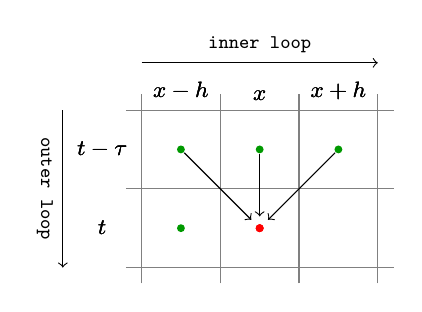
\begin{tikzpicture}
                \draw[->] (0,2.6) -- (3,2.6) node[midway,above] {\scriptsize \texttt{inner loop}};
                \draw[->] (-1,2) -- (-1,0) node[midway,rotate=270,below] {\scriptsize \texttt{outer loop} };
                \draw[step=1,gray] (-0.2,-0.2) grid (3.2,2.2);
                \begin{scope}[yshift=-5mm,xshift=-5mm]
                    \foreach \x/\y in {1/2, 2/2, 3/2, 1/1} {
                            \fill[black!40!green] (\x,\y) circle (0.5mm);
                        }
                    \foreach \x/\y in {1/2, 2/2, 3/2} {
                            \draw[->, shorten >= 1.5mm, shorten <= 0.6mm] (\x,\y) -- (2,1);

                            \fill[red] (2,1) circle (0.5mm);

                            \node at (1,2.5) [above] {\footnotesize $x-h$};
                            \node at (2,2.5) [above] {\footnotesize $x$};
                            \node at (3,2.5) [above] {\footnotesize $x+h$};
                            \node at (0,2) {\footnotesize $t-\tau$};
                            \node at (0,1) {\footnotesize $t$};
                        }
                \end{scope}
            \end{tikzpicture}
        }
        \caption{Evaluation of \texttt{V} at a single-step $x$ (i.e. the inner for-loop) in the FTCS method. All green dots are known, and red is the unknown value being evaluated.}
        \label{fig:Graphftcs}
    \end{figure}
}

\def\figBorderDD
{
    \begin{figure}[H]
        \centering
        {
            \begin{tikzpicture}
                % \draw[step=0.5cm, gray, very thin] (0,0) node[black, above=5mm] {$-L/2$} grid (8,0.5) node[black, above] {$+L/2$};
                \draw[step=0.5cm, gray, very thin] (0,0) grid (3.2,0.5);
                \draw[step=0.5cm, gray, very thin] (4.8,0) grid (8,0.5);
                \draw[|<->|] (-0.5,-0.5) -- (8.5,-0.5);
                \draw[|-|] (1,0.7) -- (1.5,0.7);
                \draw[|->] (4,-0.15) node[below] {$_o$} -- (4.5,-0.15) node[right] {$x$};
                \node at (1.25,0.7) [above] {$h$};
                \node at (-0.5,-0.5) [left] {$-L-h$};
                \node at (8.5,-0.5) [right] {$+L+h$};
                \node at (4,-0.5) [below] {$2L+2$};
                \foreach \x in {3.5,4,4.5} {
                        \foreach \y in {0.25} {
                                \fill[black] (\x, \y) circle (0.5mm);
                            }

                        \draw[step=0.5cm, gray, very thin, red] (7.99,0) grid (8.5,0.5);
                        \draw[step=0.5cm, gray, very thin, red] (-0.5,0) grid (0.01,0.5);
                    }
            \end{tikzpicture}
        }
        \caption{Discretized domain \autoref{fig:DescretizedDomain} with boundaries.}
        \label{fig:BorderDD}
    \end{figure}
}


\def\figHalo
{
    \begin{figure}[H]
        \centering
        {
            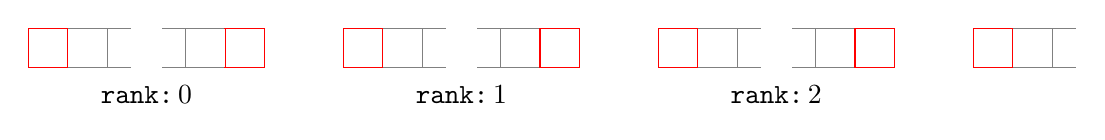
\begin{tikzpicture}
                % \draw[step=0.5cm, gray, very thin] (0,0) node[black, above=5mm] {$-L/2$} grid (8,0.5) node[black, above] {$+L/2$};
                \begin{scope}
                    \pgfmathsetmacro{\yvalb}{-2.5}
                    \pgfmathsetmacro{\yvala}{-2}

                    \foreach \x in {0,4,8,12} {
                            \begin{scope}[xshift=\x cm]
                                \draw[step=0.5cm, red] (-1.5,\yvala) grid (-1,\yvalb);
                                \draw[step=0.5cm, gray, very thin] (-0.99,\yvala) grid (-0.19,\yvalb);
                            \end{scope}
                        }

                    \foreach \x in {0,4,8} {
                            \begin{scope}[xshift=\x cm]
                                \draw[step=0.5cm, red] (0.99,\yvala) grid (1.5,\yvalb);
                                \draw[step=0.5cm, gray, very thin] (0.2,\yvala) grid (0.99,\yvalb);
                            \end{scope}
                        }
                    \foreach \x/\L in {0/0,4/1,8/2} {
                        \begin{scope}[xshift=\x cm]
                            \node at (0,\yvalb-.1) [below] {$\texttt{rank:}\, \L$};
                        \end{scope}
                    }
                \end{scope}
                % \draw[thick,->] (0,0) -- (0,-4) node[midway, fill=white, inner sep=1pt] {Text Label};

            \end{tikzpicture}
        }
        \caption{\texttt{create\_halo()} creates borders at each local discretization which is needed to implement the initial condition and sharing values.}
        \label{fig:Halo}
    \end{figure}
}

\def\figParftcs
{
    \begin{figure}[H]
        \centering
        {
            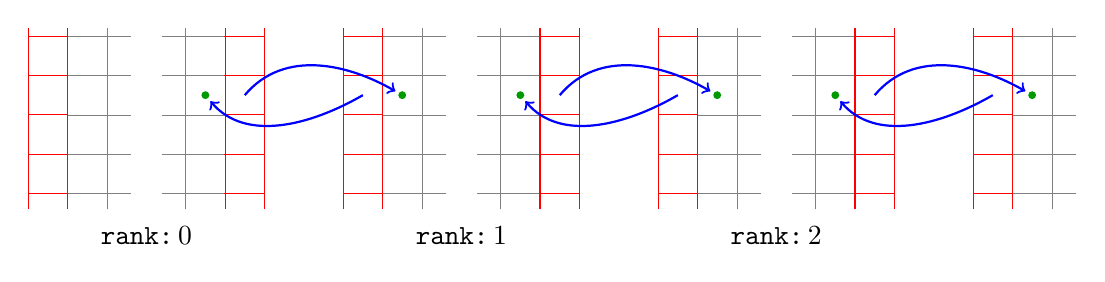
\begin{tikzpicture}
                % \draw[step=0.5cm, gray, very thin] (0,0) node[black, above=5mm] {$-L/2$} grid (8,0.5) node[black, above] {$+L/2$};

                \begin{scope}
                    \pgfmathsetmacro{\yvalb}{-4.2}
                    \pgfmathsetmacro{\yvala}{-1.9}

                    \foreach \x in {0,4,8,12} {
                            \begin{scope}[xshift=\x cm]
                                \draw[step=0.5cm, red] (-1.5,\yvala) grid (-1,\yvalb);
                                \draw[step=0.5cm, gray, very thin] (-0.99,\yvala) grid (-0.19,\yvalb);
                            \end{scope}
                        }

                    \foreach \x in {0,4,8} {
                            \begin{scope}[xshift=\x cm]
                                \draw[step=0.5cm, red] (0.99,\yvala) grid (1.5,\yvalb);
                                \draw[step=0.5cm, gray, very thin] (0.2,\yvala) grid (0.99,\yvalb);
                            \end{scope}
                        }
                    \foreach \x/\L in {0/0,4/1,8/2} {
                            \begin{scope}[xshift=\x cm]
                                \node at (0,\yvalb-.1) [below] {$\texttt{rank:}\, \L$};
                            \end{scope}
                        }

                    \foreach \x in {0,4,8} {
                            \begin{scope}[xshift=\x cm]
                                \draw[->, thick, blue, shorten >= 1mm] (1.25,-2.75) to[out=50, in=150] (3.25,-2.75);
                                \draw[->, thick, blue, shorten >= 1mm] (2.75,-2.75) to[out=-150, in=-50] (0.75,-2.75);
                                \fill[black!40!green] (3.25,-2.75) circle (0.5mm);
                                \fill[black!40!green] (0.75,-2.75) circle (0.5mm);
                            \end{scope}
                        }

                \end{scope}
            \end{tikzpicture}
        }
        \caption{Sharing of bordering values at each time-step. As \texttt{rank:0} doesn't have a left neighbour, it only performs \texttt{Sendrecv()} on the right. The last \texttt{rank} would behave similarly}
        \label{fig:Parftcs}
    \end{figure}
}

\setlength{\parindent}{0in}


\title{Term Paper – Parallelized FTCS Method}
\author{Rafay Nawaid Alvi–2132500 \& Haider Hussain–2131610}
%\date{July 2023}

\begin{document}

\maketitle

\tableofcontents
\pagebreak
\section{Introduction}

The project is to parallelize the FTCS (Forward Time Central Space) method to solve the given PDE (Partial Differential Equation) using \texttt{Python} and \texttt{mpi4py}. FTCS method is an explicit time-stepping method for numerically solving Parabolic PDEs \cite{tannehill}. The given equation is the incompressible Navier Stokes Equation, i.e. diffusion-convection equation. This particular PDE is further simplifed to a Pure-Diffusion Equation \cite{paper}.
\begin{equation}
    \displaystyle{\frac{\partial v}{\partial t} = \frac{\partial}{\partial x}\left[D(x)\frac{\partial v}{\partial x}\right]+ S(x,t)}
    \label{eq:De}
\end{equation}
Here,
\begin{table*}[h]
    \raggedright
    \begin{tabular}{rl}
        $\partial v/\partial t$ &: Rate of change of the scalar quantity $v$ \\ 
        $\partial [D(x) \frac{\partial v}{\partial x}]$/$\partial x$  &: Diffusion term \\ 
        $S(x,t)$ &: External source term
    \end{tabular}
\end{table*}

For our particular case, we will be solving the equation in (1+1)-Dimension i.e. 1 dimension in space and 1 dimension in time. For visualization, we can think of the equation to represent the rate of change of a scalar quantity $v$ (e.g. Heat, Concentration, Potential, etc.), as it spreads along the length $L$ of a 1 dimensional rod parallel to the $x$-axis as shown in \autoref{fig:Rod}



\figRod

This project will discuss the numerical solution of the equation using the serial method and most importantly the parallelized method. In the first section, we'll discuss the algorithm of the FTCS method implemented serially (i.e. using a single process or \texttt{rank}), the discretization of the equation, stability condition, the corresponding code, results, and plots.

The second section will primarily focus on the parallelization of the method, we'll use the same numerical method from the previous section, but also introduce communication between different processors. The relevant code to implement parallelization is also discussed. Finally, the results and plots of this method are compared and evaluated with the results of the first section. The last section will share the limitations and what can be done for further improvement of the current code.




\section{Serial Method}
In this section, the serial implementation of FTCS method is discussed. First the given PDE is decretized, and the initial and boundary conditions are specified. The stabilty condition is briefly touched to give reasoning on how to choose the step-sizes. Finally, the python program is revealed along with the results.
\subsection{Domain Discretization}
The numerical method that will be implemented to solve the given (1+1)-Dimensional Pure-Diffusion Equation is the FTCS (Forward Time Central Space) method. The given equation \autoref{eq:De} is discretized into \autoref{eq:Disceq}. Based on the centered space, symmetric finite differences for the space derivative was used (step-size in space $h/2$); and forward finite difference for the time derivative was used (step-size in time $\tau$).

\begin{equation}
\begin{aligned}
    v(x,t+\tau) = &v(x,t) \\
     &+ \dfrac{\tau}{h^2}D(x+h/2)[v(x+h,t) - v(x,t)] \\
     &+ \dfrac{\tau}{h^2}D(x-h/2)[v(x-h,t) - v(x,t)] \\
     &+ \tau S(x,t)
\end{aligned}
\label{eq:Disceq}
\end{equation}

The discretized domain is shown in \autoref{fig:DescretizedDomain}. This is a discretization of the same rod shown in \autoref{fig:Rod}. Note that in both figures, the centre of our 1D domain is placed at the origin $O$. With each far end of the domain being $L$ units from the origin. Each discretized cell is $h$ units.
\figDescretizedDomain

\subsection{Boundary and Initial Conditions}
\label{subsec:bic}
A key necessity to solving PDEs is the boundary and initial condition, here we use the Neumann boundaries: by setting $D(x)=0$ on the boundaries, i.e. $D(-L-h/2)=D(L+h/2)=0$ as shown in \autoref{fig:BorderDD}. The initial condition $v(x,t=0)=v_0$, $D(x)$, $S(x,t)$, the simulation time $T$ and domain length $2L$, can be given by the user in the program.

\figBorderDD

\subsection{Solution Matrix}
In order to plot the results, the value of each discretized cell ($x+h$) at each time-step ($t+\tau$) needs to be stored in solution matrix.

In our case, the solution matrix is a 2D matrix as shown in \autoref{fig:SolutionMat}, with each element representing the value of the scalar quantity $v$ at a particular time $\tau$ and space $h$. In the solution matrix, the rows represent the time-step $\tau$, and the columns represent the space-step $h$. The size of the matrix is dependent on the coarseness of the discretization. However, the domain of our solution will always be $x=[-L,L]$ and $t=[0,T]$.

\figSolutionMat

The implementation of discretizing the space and allocating the solution matrix in Python is shown below. Note that the boundaries, i.e. $-L-h$ and $L+h$ are included as well.

\begin{lstlisting}[language=Python]
# decretized space
x = np.linspace(-L-h,L+h, np.ceil(2*L/h).astype('int')+2)
N = int(T/tau)
# solution matrix including L-h/2 and L+h/2
V = np.zeros([N, np.size(x)]);
\end{lstlisting}

\subsection{Stability Condition}
The step-sizes, $h$ and $\tau$ are chosen such that accumulation of errors is prevented and the method is numerically stable. Thus we look into the stability condition. For the FTCS method of a 1D Parabolic PDE of the form $\frac{\partial u(x, t)}{\partial t} = \alpha \frac{\partial^2 u(x, t)}{\partial x^2}$, the following condition must be satisfied \cite{griffiths}.
\begin{equation}
    \dfrac{\tau}{h^2} \leq \dfrac{1}{2 \alpha}
    \label{eq:Stabilitycondition}
\end{equation}

In our given differential equation, there's no scalar coefficient, hence, $\alpha=1$. By fixing the value of $\tau$, we can then determine the least step-size $h$, and hence the maximum number of discretized cells in our domain, i.e. columns of the solution matrix, is also determined.

\vspace{1mm}
\textbf{Example:} Let us fix $\tau = 0.001$, and determine the minimum value for $h$ and the corresponding number of discretized cells. Continuing from \autoref{eq:Stabilitycondition}. 


\begin{equation}
    \begin{aligned}
        h&\geq\sqrt{2\tau} \\
        h&\geq\sqrt{2\cdot 0.001} \\ 
        h&\geq\frac{\sqrt{5}}{50} \quad (\text{where } \frac{\sqrt{5}}{50} \approx 0.0447)
    \end{aligned}
    \label{eq:Min_h}
\end{equation}
We can now determine the appropriate number of discretized cells of our domain ($\text{\#cols}$). Using the inequality obtained from \autoref{eq:Min_h} into the relationship $h = \frac{2L}{\text{\#cols}}$ from \autoref{fig:SolutionMat}.
\begin{equation}
    \begin{aligned}
        \frac{2L}{\text{\#cols}} &\geq \frac{\sqrt{5}}{50} \\
        \text{\#cols} &\leq \frac{2\cdot5}{\sqrt{5}/50}\\
        \text{\#cols} &\leq 100\sqrt{5} \quad (\text{where } 100\sqrt{5} \approx 223.6)
    \end{aligned}
\end{equation}
The similar approach can be done for finer values as well, \autoref{tab:Coarsness} below shows the values for $h$ and \#cols for various $\tau$ values.
\begin{table}[H]
    \centering
    \renewcommand{\arraystretch}{1.5}
    \begin{tabular}{|c|c|c|}
        \hline
        For $\tau = 1\times10^{-1}$ & $h \geq 0.1414$ & $\text{\#cols}\leq70.7$ \\
        \hline
        For $\tau = 1\times10^{-2}$ & $h \geq 0.0447$ & $\text{\#cols}\leq223.6$ \\
        \hline
        For $\tau = 1\times10^{-3}$ & $h \geq  0.0141$ & $\text{\#cols}\leq707.1$ \\
        \hline
        For $\tau = 1\times10^{-4}$ & $h \geq  0.0044$ & $\text{\#cols}\leq2236.1$ \\
        \hline
    \end{tabular}
    \caption{$\tau$ and $h$ that satisfy the stability condition \autoref{eq:Stabilitycondition}, and the corresponding \#cols for the solution matrix (i.e. the number of discretized cells in space) }
    \label{tab:Coarsness}
\end{table}

It should be noted that the size of the entire solution matrix would increase pretty quickly with finer values of $\tau$ or $h$. For our demonstration, we will henceforth only work with $\tau = 0.001$ and $\tau=0.0001$.

\subsection{Python Program (Serial)}
The following section will solve the FTCS method using a single processor. The parameters $2L$ for the domain length and $T$ for the simulation time are specified. The desired coarseness $h$ is chosen based on the value of $\tau$ and in accordance with the stability condition \autoref{eq:Stabilitycondition}. The program is run for two cases $\tau = 0.001$ and $\tau=0.0001$ respectively. The following parameters are fixed for each case:

\begin{table*}[h]
    \renewcommand{\arraystretch}{1}
\begin{tabular}{rl}
    $2L =$&$10$ \\
    $T =$&$2$ \\
    $h =$&$2L/\text{cols}$
\end{tabular}
\end{table*}

Thus specifiying our domain to $-5\leq x \leq 5$ and $0\leq t \leq 2$. Next, $\tau$ and $h$ are chosen based on the information from \autoref{tab:Coarsness}.
\begin{table*}[h]
    \centering
    \renewcommand{\arraystretch}{1}
\begin{tabular}{l|l}
    \textbf{case 1}  & \textbf{case 2} \\ 
    $\tau = 0.001$ & $\tau = 0.0001$\\
    cols = 223 $\implies$ $h=0.0448$  & cols = 707 $\implies$ $h=0.0141$
\end{tabular}
\end{table*}


\vspace{1mm}
The initial condition
$v_0 = 
\begin{cases}
1 & \text{if } |x|<1.5 \\
0 & \text{else }
\end{cases}
$. $D$ and $S$ are initialized as
\begin{lstlisting}[language=Python]
v0 = lambda x   : float(abs(x)<1.5);
D  = lambda x   : 1 
S  = lambda x,t : 0 
\end{lstlisting}

The numerical method begins by assigning the initial values in the solution matrix \texttt{V}.
\begin{lstlisting}[language=Python]
for l in range(np.size(x)):
    V[0,l] = v0(x[l])
\end{lstlisting}

The following code is the FTCS method. This is the direct translation of the discretized equation \autoref{eq:Disceq} to Python. The variables \texttt{Dp} and \texttt{Dm} represent the value of the coefficient $D(x)$ evaluated at $D(x+h/2)$ and $D(x-h/2)$, and it is $D(x) = 0$ at the borders as discussed in \autoref{subsec:bic}.

\begin{lstlisting}[language=Python]
for lt in range(1,N):
    for lx in range(1,np.size(x)-1):
        # evaluate D at lx
        Dp = D(x[lx]+h/2) * (np.abs(x[lx]+h/2)<L)
        Dm = D(x[lx]-h/2) * (np.abs(x[lx]-h/2)<L)

        V[lt,lx] = V[lt-1,lx] + (tau/h**2)*Dp*((V[lt-1,lx+1]) - V[lt-1,lx])+\
                                (tau/h**2)*Dm*((V[lt-1,lx-1]) - V[lt-1,lx])+\
                                tau*S(x[lx], -(lt-1)*tau)
\end{lstlisting}
From the for-loops, we can see that to evaluate \texttt{V} at every step in \texttt{lt} i.e. \texttt{V[lt,lx]}, the values of \texttt{V} at locations \texttt{lx-1, lx, lx+1} from the previous time-step \texttt{lt-1} must be known as shown in \autoref{fig:Graphftcs}.

\graphftcs

\subsection{Program Files}
The directory \texttt{serial\_diffusion} contains files to run the program as shown in \autoref{fig:Serialdir}. To run, execute the command: \texttt{\$ python main.py}.
\begin{figure}[H]
    \centering
    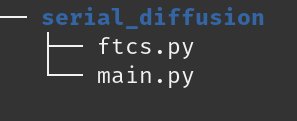
\includegraphics[width=0.3\textwidth]{figures/serial_dir0.png}
    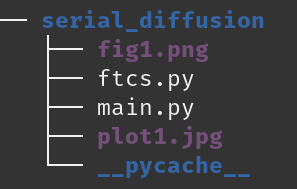
\includegraphics[width=0.3\textwidth]{figures/serial_dir1.png}
    \caption{Contents within serial directory before and after running \texttt{main.py}}
    \label{fig:Serialdir}
\end{figure}
% \vspace{-0.5cm}
The user inputs are intialized as:
\begin{lstlisting}[language=Python]
L = 5
T = 2
h = (2*L)/223 # or (2*L)/707
tau = 0.001 # or 0.0001
\end{lstlisting}

\subsection{Results}
\label{subsec:results}
Currently, we are interested in knowing if our implementation is correct. Fortunately, for our 1D problem, \autoref{eq:De}, there exists an analytical solution:
\begin{equation}
    v(x,t) = \dfrac{1}{2}\left[ \text{erf}\left( \dfrac{1.5 - x}{2\sqrt{Dt}} \right) - \text{erf}\left( \dfrac{-1.5 - x}{2\sqrt{Dt}} \right) \right] 
    \label{eq:An}
\end{equation}
Here, the error-function $\text{erf}(z) = \frac{2}{\pi}\int_{0}^{z}e^{-y^2} \text{d}y$. This error-function can be used in Python through the SciPy library: \texttt{scipy.special.erf()}

To verify our implementation, we can easily plot our solution obtained through the FTCS method against the analytical solution \autoref{eq:An}. Below are both solutions for $v(x,t)$ plotted at different times $t$.

\begin{figure}[H]
    \centering
    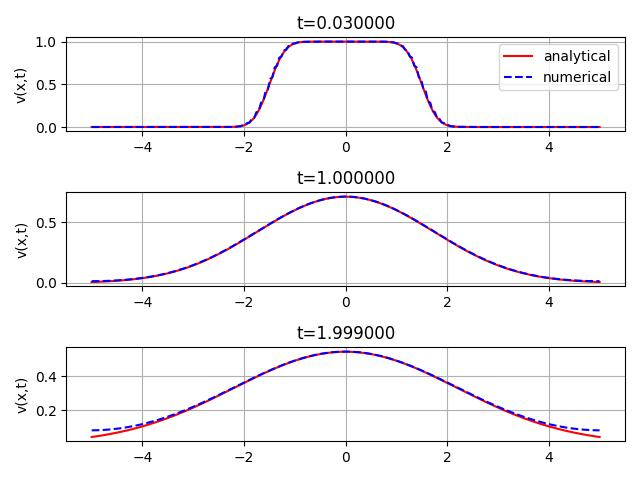
\includegraphics[width=0.6\textwidth]{figures/serial_plot.jpg}
    \caption{Comparison of the solutions obtained analytically (red) and FTCS method (dashed blue)}
    \label{fig:SerialResult}
\end{figure}

We can see in \autoref{fig:SerialResult} that our numerical method performs really well, specially for times $t \ll T$.

The execution times for the numerical method for each case $\tau$ are:
\begin{table}[H]
    \centering
\begin{tabular}{|c|c|c|c|c|}
    \hline
    & $\tau$ & $h$ &  solution matrix \texttt{V} & execution time $[s]$ \\
    \hline
    case 1 & $1\times10^{-2}$ & 0.0448 & 2000 $\times$ 223 & 5.83 \\
    case 2& $1\times10^{-3}$ & 0.0014 & 20000 $\times$ 707 & 187.27 \\
    \hline
\end{tabular}
\caption{Execution times for each case. The size of \texttt{V} significantly increases with finer $\tau$ and $h$, thus increasing execution times. These programs were executed in the \textbf{stromboli} environment}
\end{table}



\pagebreak
\section{Parallel Method}
This section modifies the implementation done in the previous section such that numerical method is run by more than a single processor. The main idea is to divide the domain from \autoref{fig:DescretizedDomain} and distribute it to a certain number of processors. Since each processor has one chunk of the entire domain, they can all locally solve for their domains simultaneously and combine the results, resulting in a significant decrease in the total execution time. In Python, this approach makes use of the MPI (Message Passing Interface) module \texttt{mpi4py}.

In accordance with convention, the terminology \texttt{rank} will be used to refer to individual processes. And to keep things easier, the \texttt{size} (i.e. the total number of \texttt{ranks}) is chosen to always be a power of 2, i.e. $\texttt{size}= 2^r$, where $ r\in \mathbb{N}_{0}$ (non-negative integer).

\subsection{Domain Decomposition}
Since the domain needs to be divided evenly among $2^r$ \texttt{ranks}, the \#cols must be divisible by every \texttt{size} $2^r$. Let us now estimate the appropriate $h$ that generates \#cols such that they can be evenly divided among $2^r$ \texttt{ranks}.

\textbf{Example:} Let us fix  $\tau=0.001$. From \autoref{tab:Coarsness}, we know $h\geq0.0447$ and consequently we selected the maximum possible $\#\text{cols}=223$. In this case, 223 cannot be evenly divided into $2^r$ \texttt{ranks}, so we choose the nearest power of 2 to be our column size. Let us denote all such \#cols: $2^r \leq 223$ in a set $S_1$.
\begin{equation}
    \begin{aligned}
S_1 = \{2^r \mid 2^r \leq \text{max(\#\text{cols})}, r \in \mathbb{N}_{0} \}
    \end{aligned}
\end{equation}

For max($\#\text{cols})=223$, $S_1$ becomes:
\begin{equation}
    \begin{aligned}
        S_1 &= \{2^r \mid 2^r \leq 223, r \in \mathbb{N}_{0} \}  \\ 
        &= \{ 1,2,4,8,16,32,64,128 \} 
    \end{aligned}
    \label{eq:ddt31}
\end{equation}
$S_1$ contains all \#cols that are divisible by every $\texttt{size}=2^r\leq223$, and the maximum \#cols we can now use is $\text{max}(S_1) = 128$, which is significantly less than 223 from our serial attempt.

To improve on \#cols, let us also fix the maximum $\texttt{size}=2^k=64$. With this we can now increase the column size to a number that is a multiple of 64 and also satisfies $\#\text{cols}\leq223$. Let us denote all such \#cols: $\text{max}(S_1) \leq 64\cdot p \leq 223$ in a set $S_2$. 
\begin{equation}
    \begin{aligned}
        S_2 = \{2^k \cdot p \mid \text{max}(S_1) \leq 2^k \cdot p \leq \text{max(\#\text{cols})},p \in \mathbb{N}_0\}
    \end{aligned}
\end{equation}
For max($\#\text{cols})=223$ and $2^k=64$, $S_2$ becomes:
\begin{equation}
    \begin{aligned}
        S_2 &= \{64 \cdot p \mid 128 \leq 64\cdot p \leq 223,p \in \mathbb{N}_0\} \\
        &= \{128, 192\}
    \end{aligned}
    \label{eq:ddt32}
\end{equation}

The $\text{max}(S_2)$ would be the maximum \#cols for our solution matrix, given a $\tau$ and a specified max number of ranks, i.e $\texttt{size}=2^k$.
\begin{equation}
    \begin{aligned}
        \#\text{cols} &= \text{max}(S_2) \\
         &= 192 \implies h = 0.052 \quad\quad \because  h=\dfrac{2L}{\text{\#cols}}
    \end{aligned}
\end{equation}

To summarise, given $\tau=0.001$ and \texttt{sizes} $2^{k} \leq 64$, the domain is discretized to 192 cells, i.e. $\text{max}(\#\text{cols})=192$ which can be evenly distributed to all \texttt{ranks} as shown in \autoref{tab:DomainDecomposition1}.

\begin{table}[H]
    \centering
    \begin{tabular}{|c|c|c|c|c|c|c|c|}
        \hline
        $\texttt{size}=2^k$ & 1 & 2 & 4 & 8 & 16 & 32 & 64 \\
        \hline
        \#cols per \texttt{rank} & 192 & 96 & 48 & 24 & 12 & 6 & 3 \\
        \hline
    \end{tabular}
    \caption{Domain decomposition for \texttt{sizes}: $2^k\leq64$ and $\tau=0.001$}
    \label{tab:DomainDecomposition1}
\end{table}

Similarly, for $\tau=0.0001$ and $\texttt{sizes } 2^k\leq64$, we will have the following:
\begin{equation}
\begin{aligned}
    S_1 &= \{1,2,4,8,16,32,64,128,256,512 \}  \\
    S_2 &= \{512,578,640,704 \} \\
    \text{max}(S_2) &= 704 \implies h = 0.014 \quad\quad \because h=\dfrac{2L}{\text{\#cols}}
\end{aligned}
\label{eq:ddt4}
\end{equation}
\begin{table}[H]
    \centering
    \begin{tabular}{|c|c|c|c|c|c|c|c|}
        \hline
        $\texttt{size}=2^k$ & 1 & 2 & 4 & 8 & 16 & 32 & 64 \\
        \hline
        \#cols per \texttt{rank} & 704 & 352 & 176 & 88 & 44 & 22 & 11 \\
        \hline
    \end{tabular}
    \caption{Domain decomposition for \texttt{sizes}: $2^k\leq64$ and $\tau=0.0001$}
    \label{tab:DomainDecomposition2}
\end{table}

The way the domain would be decomposed using MPI is as follows:
\begin{lstlisting}[language=Python]
# allocate space of local_x in all ranks
x = np.zeros(global_array_size//size) 
if rank == 0:
    h = (2*L/global_array_size)
    # discretization of the entire space 2L
    global_x = np.linspace(-L,L, np.ceil(2*L/h).astype('int'))
else:
    # initialize the variables in all other ranks to 0.
    global_x = np.zeros(1)
    h = 0

# distribution of global_x to all ranks
comm.Scatter(global_x, x, root = 0) 
\end{lstlisting}

Here, \texttt{global\_x} is the total discretization of the entire domain and it only exist in \texttt{rank=0}, it is distributed to each \texttt{rank} in their local variable \texttt{x}. This decomposition of the domain is done using \texttt{Scatter()}, the working of which is demonstrated in \autoref{fig:DDecompose}. Also, the value for \#cols is defined in \texttt{global\_array\_size} which is used to initialize \texttt{h}. 

\figDDecompose

\subsection{Communication}
Since each \texttt{rank} has an equally divided part of the entire domain, it is required that they all implement the FTCS method locally and simultaneously. In order for this to work, each \texttt{rank} must be able to share its bordering values with its neighbouring \texttt{rank}. So we introduce a \textit{halo} around each local discretization \texttt{local\_mat} as shown in \autoref{fig:Halo}.

\begin{lstlisting}[language=Python]
def create_halo(local_mat: np.ndarray, h: float):
    # ...
    local_mat = np.r_[local_mat[0]-h, local_mat, local_mat[-1] + h]
    return local_mat
\end{lstlisting}

\figHalo

At each rank, \texttt{create\_halo()} concatenates one step after and one step before the local discretized \texttt{x}. This ensures that the bordering values of each rank are overlapped, which is useful for implementing the initial condition and storing the values as boundaries to perform FTCS (as shown in \autoref{fig:Graphftcs}). Furthermore, the solution matrix is allocated at each rank.
\begin{lstlisting}[language=Python]
x = create_halo(x,h)
V = np.zeros([N, np.size(x)]) 
\end{lstlisting}

After each time-step of the FTCS method, each \texttt{rank} should have a new row of calculated \texttt{V[lt,:]} values in its local solution matrix \texttt{V}. It will then \textit{send} its the bordering values of the solution matrix to its neighbouring \texttt{ranks} on the left and right, and also \textit{receive} the bordering values of the neighbouring \texttt{ranks}. This can be done using \texttt{Sendrecv()}

\begin{lstlisting}[language=Python]
# send and receive from left rank
if rank > 0:
    comm.Sendrecv(sendleft, rank - 1, 0, recvleft, rank - 1)
# send and receive from right rank
if rank < size - 1:
    comm.Sendrecv(sendright, rank + 1, 0,recvright, rank + 1)
\end{lstlisting}

The above code is a snippet of a user-defined function \texttt{exchange\_vals()}, that is used in the parallelized FTCS method shown below.

\begin{lstlisting}[language=Python]
# ftcs method
for lt in range(1,N):
    V = exchange_vals(V,lt)
    for lx in range(1,np.size(x)-1):
        Dp = D(x[lx]+h/2) * (np.abs(x[lx]+h/2)<L)
        Dm = D(x[lx]-h/2) * (np.abs(x[lx]-h/2)<L)

        V[lt,lx] = V[lt-1,lx] + (tau/h**2)*Dp*((V[lt-1,lx+1]) - V[lt-1,lx])+\
                                (tau/h**2)*Dm*((V[lt-1,lx-1]) - V[lt-1,lx])+\
                                 tau*S(x[lx], -(lt-1)*tau)
\end{lstlisting}

This is the FTCS method that is implemented locally and simultaneously by every \texttt{rank} to solve for their own solution matrix. It can be seen from \autoref{fig:Parftcs} that each rank \texttt{sends} a value from their borders, but \texttt{receives} a value into its solution matrix.

\figParftcs

Finally, once the numerical method is completed, all of the solution matrices are combined back at \texttt{rank=0} into a complete solution matrix (like \autoref{fig:SolutionMat}) using \texttt{gather()}.

\begin{lstlisting}
global_V = comm.gather(V, root = 0)
\end{lstlisting}

\subsection{Project Files and Submissions to SLURM}
The intent is to generate strong scaling plots, i.e. we need to observe how the execution time for the FTCS method speeds up with increase in number of processors, i.e. $\texttt{sizes}\leq2^r$ compared to $\texttt{size}=1$. And we also need to observe the execution times for increasing $h$ and $\tau$.

To conduct these simulations, we have divided the project in two cases:

\vspace{1mm}
\textbf{Case1: $\tau=0.001$}

Here, we will work with the domain decompositions shown in \autoref{tab:DomainDecomposition1}. Additionally, the discretization step $h$ is also varied to show the execution times for each case. The other discretization steps used are from the set $S_1 \cup S_2 = S$ from \autoref{eq:ddt31} and \autoref{eq:ddt32}. However we are only interested in values that keep $h \leq 1.5$ so as to keep a somewhat reasonable discretization. This amounts to values: 

\begin{equation}
    \begin{aligned}
    S_{\geq8} &= \{x| x \in S, x \geq 8\}  \\ 
    &= \{ 8,16,32,64,128,192 \}
    \end{aligned}
\end{equation}

\begin{table}[H]
    \centering
    \begin{tabular}{|c|c|c|c|c|c|c|c|c|}
        \hline
        $\texttt{size}=2^k$ & 1 & 2 & 4 & 8 & 16 & 32 & 64 & $h = \frac{2L}{\text{\#cols}}$\\
        \hline
        \#cols per \texttt{rank} & 192 & 96 & 48 & 24 & 12 & 6 & 3 & $ 0.052$\\
        \hline
        \#cols per \texttt{rank} & 128 & 64 & 32 & 16 & 8 & 4 & 2 & $0.078$\\
        \hline
        \#cols per \texttt{rank} & 64 & 32 & 16 & 8 & 4 & 2 & 1 & $0.156$ \\
        \hline
        \#cols per \texttt{rank} & 32 & 16 & 8 & 4 & 2 & 1  & - & $0.312$\\
        \hline
        \#cols per \texttt{rank} & 16 & 8 & 4 & 2 & 1  & - & - & $0.625$\\
        \hline
        \#cols per \texttt{rank} & 8 & 4 & 2 & 1 & -  & - & - & $1.250$\\
        \hline
    \end{tabular}
    \caption{All 36 subcases for Case1: $\tau=0.001$}
\end{table}

Similarly for \textbf{Case2: $\tau=0.0001$}

The domain decompositions are taken from \autoref{tab:DomainDecomposition2}. The discretizations are from $S_1 \cup S_2 = S$ from \autoref{eq:ddt4}.
\begin{equation}
    \begin{aligned}
        S_{\geq8} = \{8,16,32,64,128,256,512,570,578,640,704\}
    \end{aligned}
\end{equation}


\begin{table}[H]
    \centering
    \begin{tabular}{|c|c|c|c|c|c|c|c|c|}
        \hline
        $\texttt{size}=2^k$ & 1 & 2 & 4 & 8 & 16 & 32 & 64 & $h = \frac{2L}{\text{\#cols}}$\\
        \hline
        \#cols per \texttt{rank} & 704 & 352 & 176 & 88 & 44 & 22 & 11 & $0.014$ \\ 
        \hline
        \#cols per \texttt{rank} & 640 & 320 & 160 & 80 & 40 & 20 & 10 & $0.016$ \\ 
        \hline
        \#cols per \texttt{rank} & 578 & 289 & 144 & 72 & 36 & 18 & 9 & $0.017$ \\ 
        \hline
        \#cols per \texttt{rank} & 512 & 256 & 128 & 64 & 32 & 16 & 8 & $0.020$ \\ 
        \hline
        \#cols per \texttt{rank} & 256 & 128 & 64 & 32 & 16 & 8 & 4 & $0.039$ \\ 
        \hline
        \#cols per \texttt{rank} & 128 & 64 & 32 & 16 & 8 & 4 & 2 & $0.078$ \\ 
        \hline
        \#cols per \texttt{rank} & 64 & 32 & 16 & 8 & 4 & 2 & 1 & $0.156$ \\ 
        \hline
        \#cols per \texttt{rank} & 32 & 16 & 8 & 4 & 2 & 1 & - & $0.312$ \\ 
        \hline
        \#cols per \texttt{rank} & 16 & 8 & 4 & 2 & 1 & - & - & $0.625$ \\ 
        \hline
        \#cols per \texttt{rank} & 8 & 4 & 2 & 1 & - & - & - & $1.250$ \\ 
        \hline
    \end{tabular}
    \caption{All 64 subcases for Case1: $\tau=0.0001$}
\end{table}

The directory \texttt{parallel\_diffusion} contains the files to run the program. The program is ran in the \textbf{stromboli} cluster environment provided by Bergische Universität Wuppertal (BUW). The following commands are executed within this folder to run the program:
\begin{lstlisting}[language=sh]
$ module load tools/anaconda3/
$ python main.py
\end{lstlisting}

\begin{figure}[H]
    \centering
    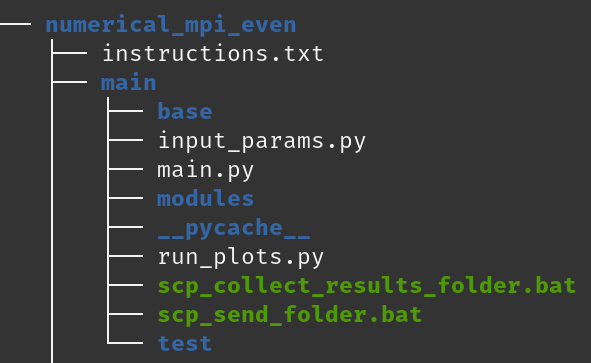
\includegraphics[width=0.45\textwidth]{figures/parallel_dir0.png}
    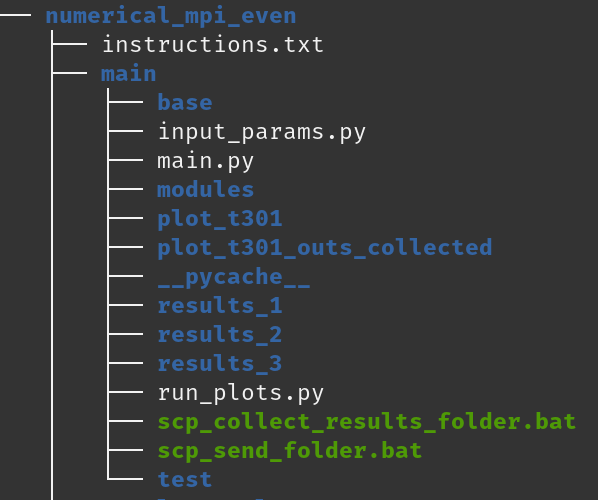
\includegraphics[width=0.45\textwidth]{figures/parallel_dir1.png}
    \caption{Contents within the directory before and after running \texttt{main.py}}
\end{figure}

The \texttt{base/} directory contains \texttt{ftcs.py} file with additional functionalities to enable parallelization. \texttt{main.py} copies the \texttt{base/} to the \texttt{results\_*/} directories, with the parameters $\tau$, $h$ and \texttt{size} initialized for each particular subcase.

\begin{figure}[H]
\begin{lstlisting}[language=Python]
copy_files_base_to_case()

node = assign_node() # assign appropriate node

modify_case_params() # modification of parameters in each case

run_case() # run case inside each case directory
\end{lstlisting}
\caption{Functions inside \texttt{main.py} to illustrate the automation}
\label{fig:mainpy}
\end{figure}

This is \texttt{repeated} 3 times, as indicated in \autoref{fig:inputparams}, resulting in the directories \texttt{results\_1/}, \texttt{results\_2/}, and \texttt{results\_3/}. Each \texttt{results} folder contains all simulations for a given $\tau$ with similar plots as \autoref{fig:SerialResult}. The parameters for a different $\tau$ can be changed in \texttt{input\_params.py}.

\begin{figure}[H]
\begin{lstlisting}[language=Python]
# USER INPUT for tau = 0.0001
tau = 0.0001
x_divs = [8, 16, 32, 64, 128, 256, 512, 576, 640, 704]
procs  = [1,2,4,8,16,32,64]
repeat = 3
delta_t = "plot_t401"
\end{lstlisting}
\caption{Snippet from \texttt{input\_params.py} showing user input}
\label{fig:inputparams}
\end{figure}

The process of submitting each case through \texttt{SLURM} is automated in \texttt{script\_main.py} found inside \texttt{modules/}, these functions are utitlized in \texttt{main.py} as shown in \autoref{fig:mainpy}. This also makes sure that the appropriate \texttt{nodes} are selected based on the amount of processors used. To avoid overloading, a new case is submitted once the previous is completed or the program at least waits a certain amount of time before submitting.

\begin{lstlisting}[language=Python]
os.system("sbatch submit_script.sh")
\end{lstlisting}

After execution, the program also prompts to run \texttt{run\_plots.py} to generate the relevant plots. This program can be run separately as well, provided the \texttt{results\_*} folders exist and the parameters provided in \texttt{input\_params.py} are not changed.
\begin{lstlisting}[language=sh]
$ python run_plots.py
\end{lstlisting}

\subsection{Scalability Plot: Strong Scaling}
Since we are already sure about the correctness of the program from \autoref{subsec:results} because we're using the same implementation of the FTCS from the serial section. Here, we will be mostly focusing on the performance of our parallelization, i.e. the time taken to execute the numerical method in relation with the amount of processes used. The plots shown in this section are the strong scaling plots and the comparion of execution times for all cases from \autoref{tab:DomainDecomposition1} and \autoref{tab:DomainDecomposition2}.

For the strong scaling, the size of the problem is kept constant, and the Speed-up$(\frac{t_n}{t_1})$ is observed in relation with the increase in the number of processes (i.e \texttt{size}). Here, the speed-up is the ratio of $t_n$ (the execution time for $n$ processes) to $t_1$ (execution time for 1 process or the serial process).

\begin{figure}[H]
    \centering
    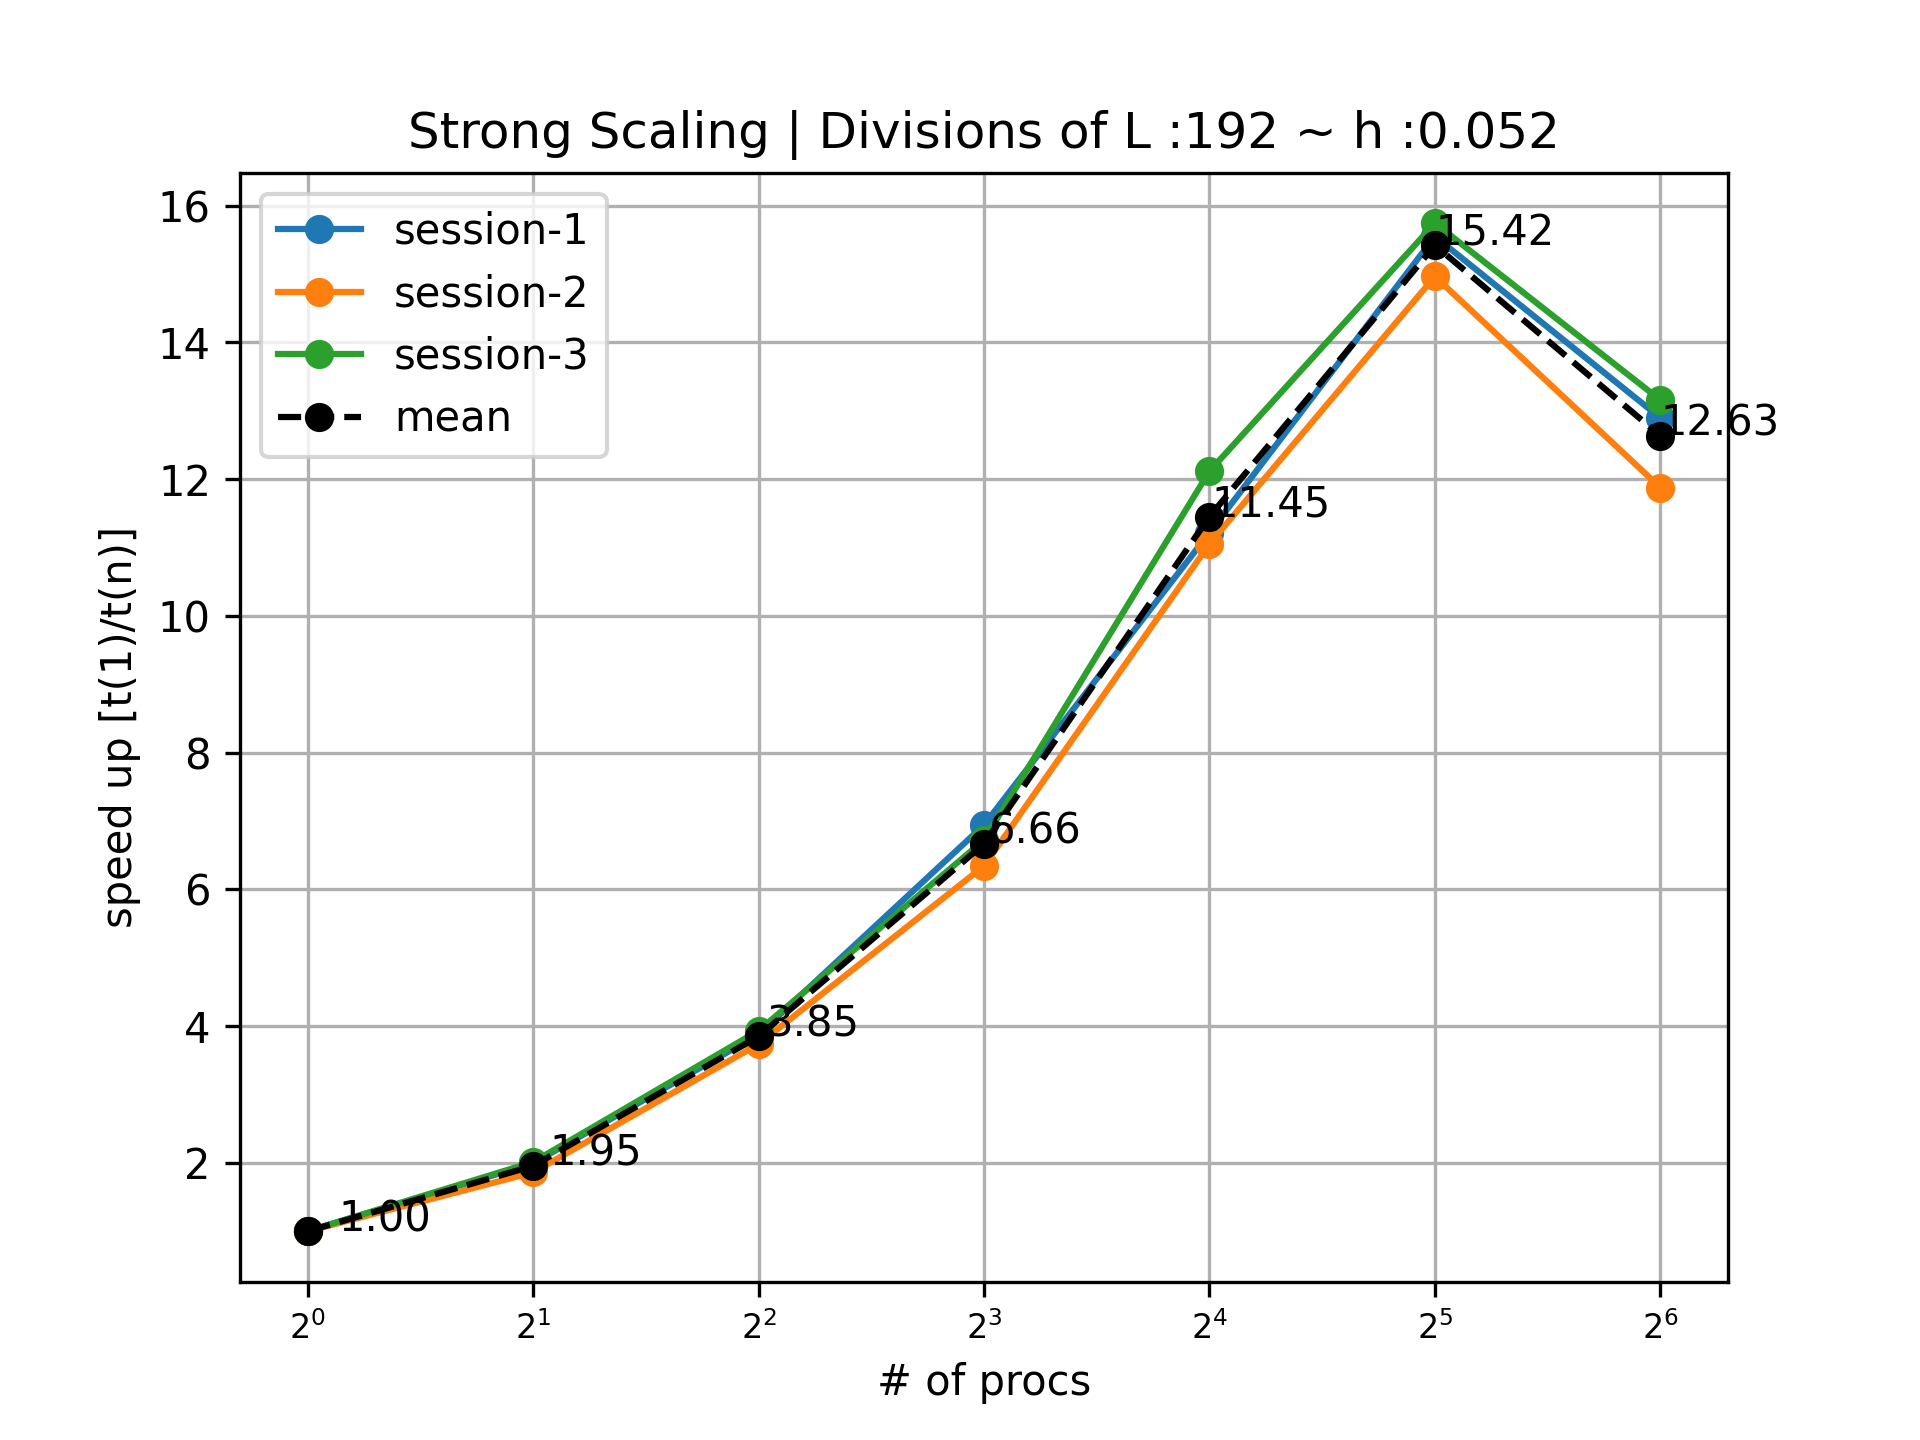
\includegraphics[width=0.7\textwidth]{figures/t301_scaling192-plot.png}
    \caption{Strong Scaling Plot for $\tau=0.001$, this shows the speed up in time with increase in \texttt{size}}
    \label{fig:t301scaling}
\end{figure}
The plots in \autoref{fig:t301scaling} and \autoref{fig:t401scaling} show the speed up in the execution time with increase in the number of processes. It can be observed that with each successive power of 2 in the number of processes, the speed-up nearly doubles from the previous step. 

The sudden decrease in speed-up at the end can be explained by the fact that the overall communication between a large a number of processes is significantly more than the local problem size within each process. Thus, regardless of the speed of the numerical method, the high communication overhead between processes slows down the overall performance.

\begin{figure}[H]
    \centering
    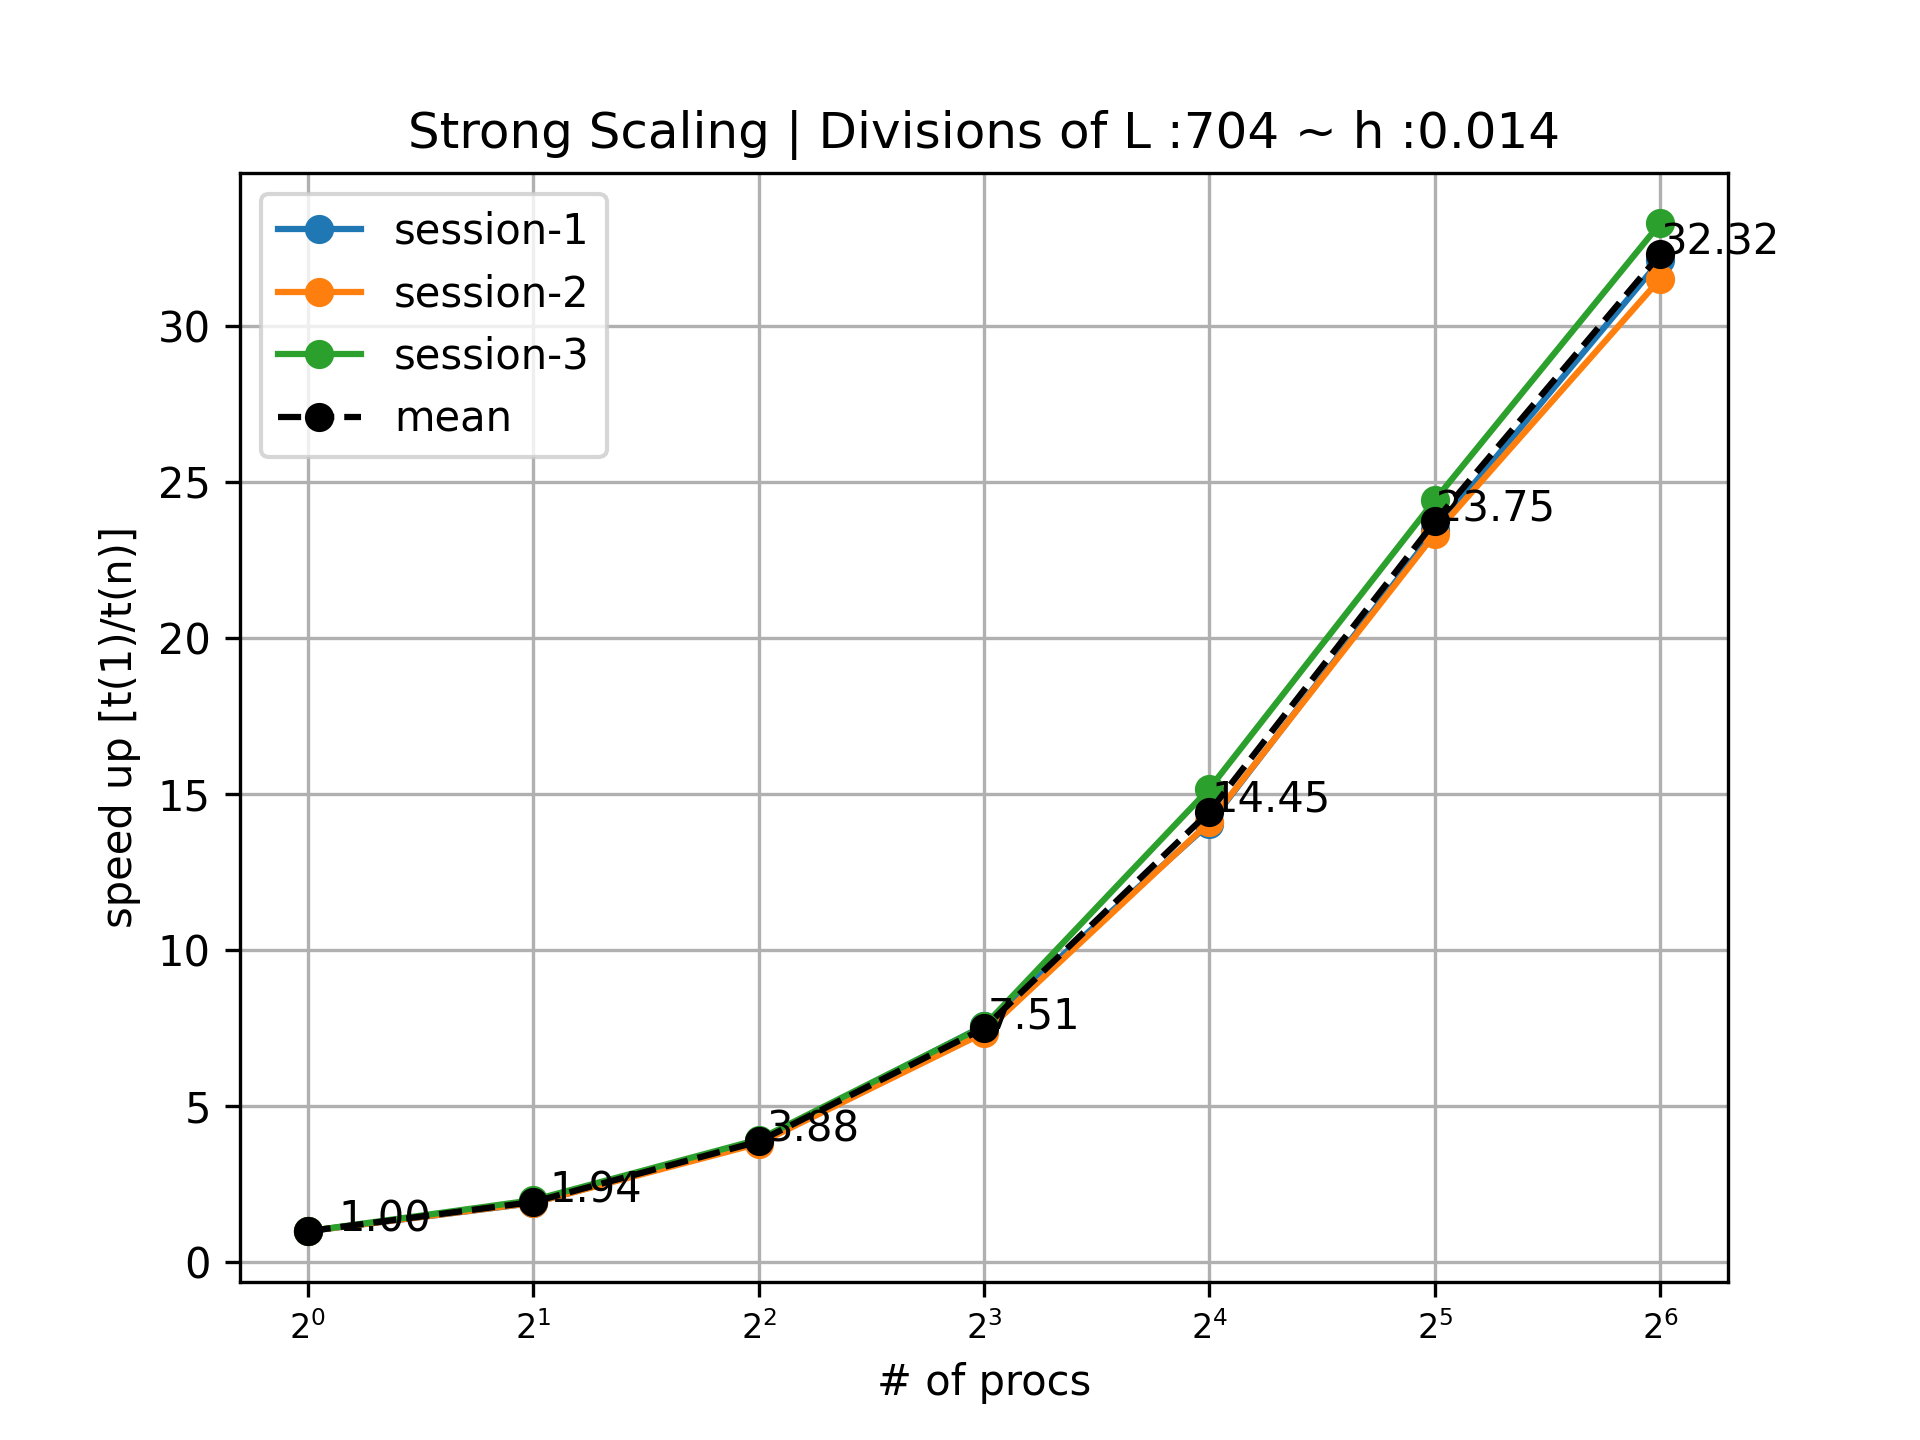
\includegraphics[width=0.7\textwidth]{figures/t401_scaling704-plot.png}
    \caption{Strong Scaling Plot for $\tau=0.0001$, this shows the speed up in time with increase in \texttt{size}}
    \label{fig:t401scaling}
\end{figure}


\begin{figure}[H]
    \centering
    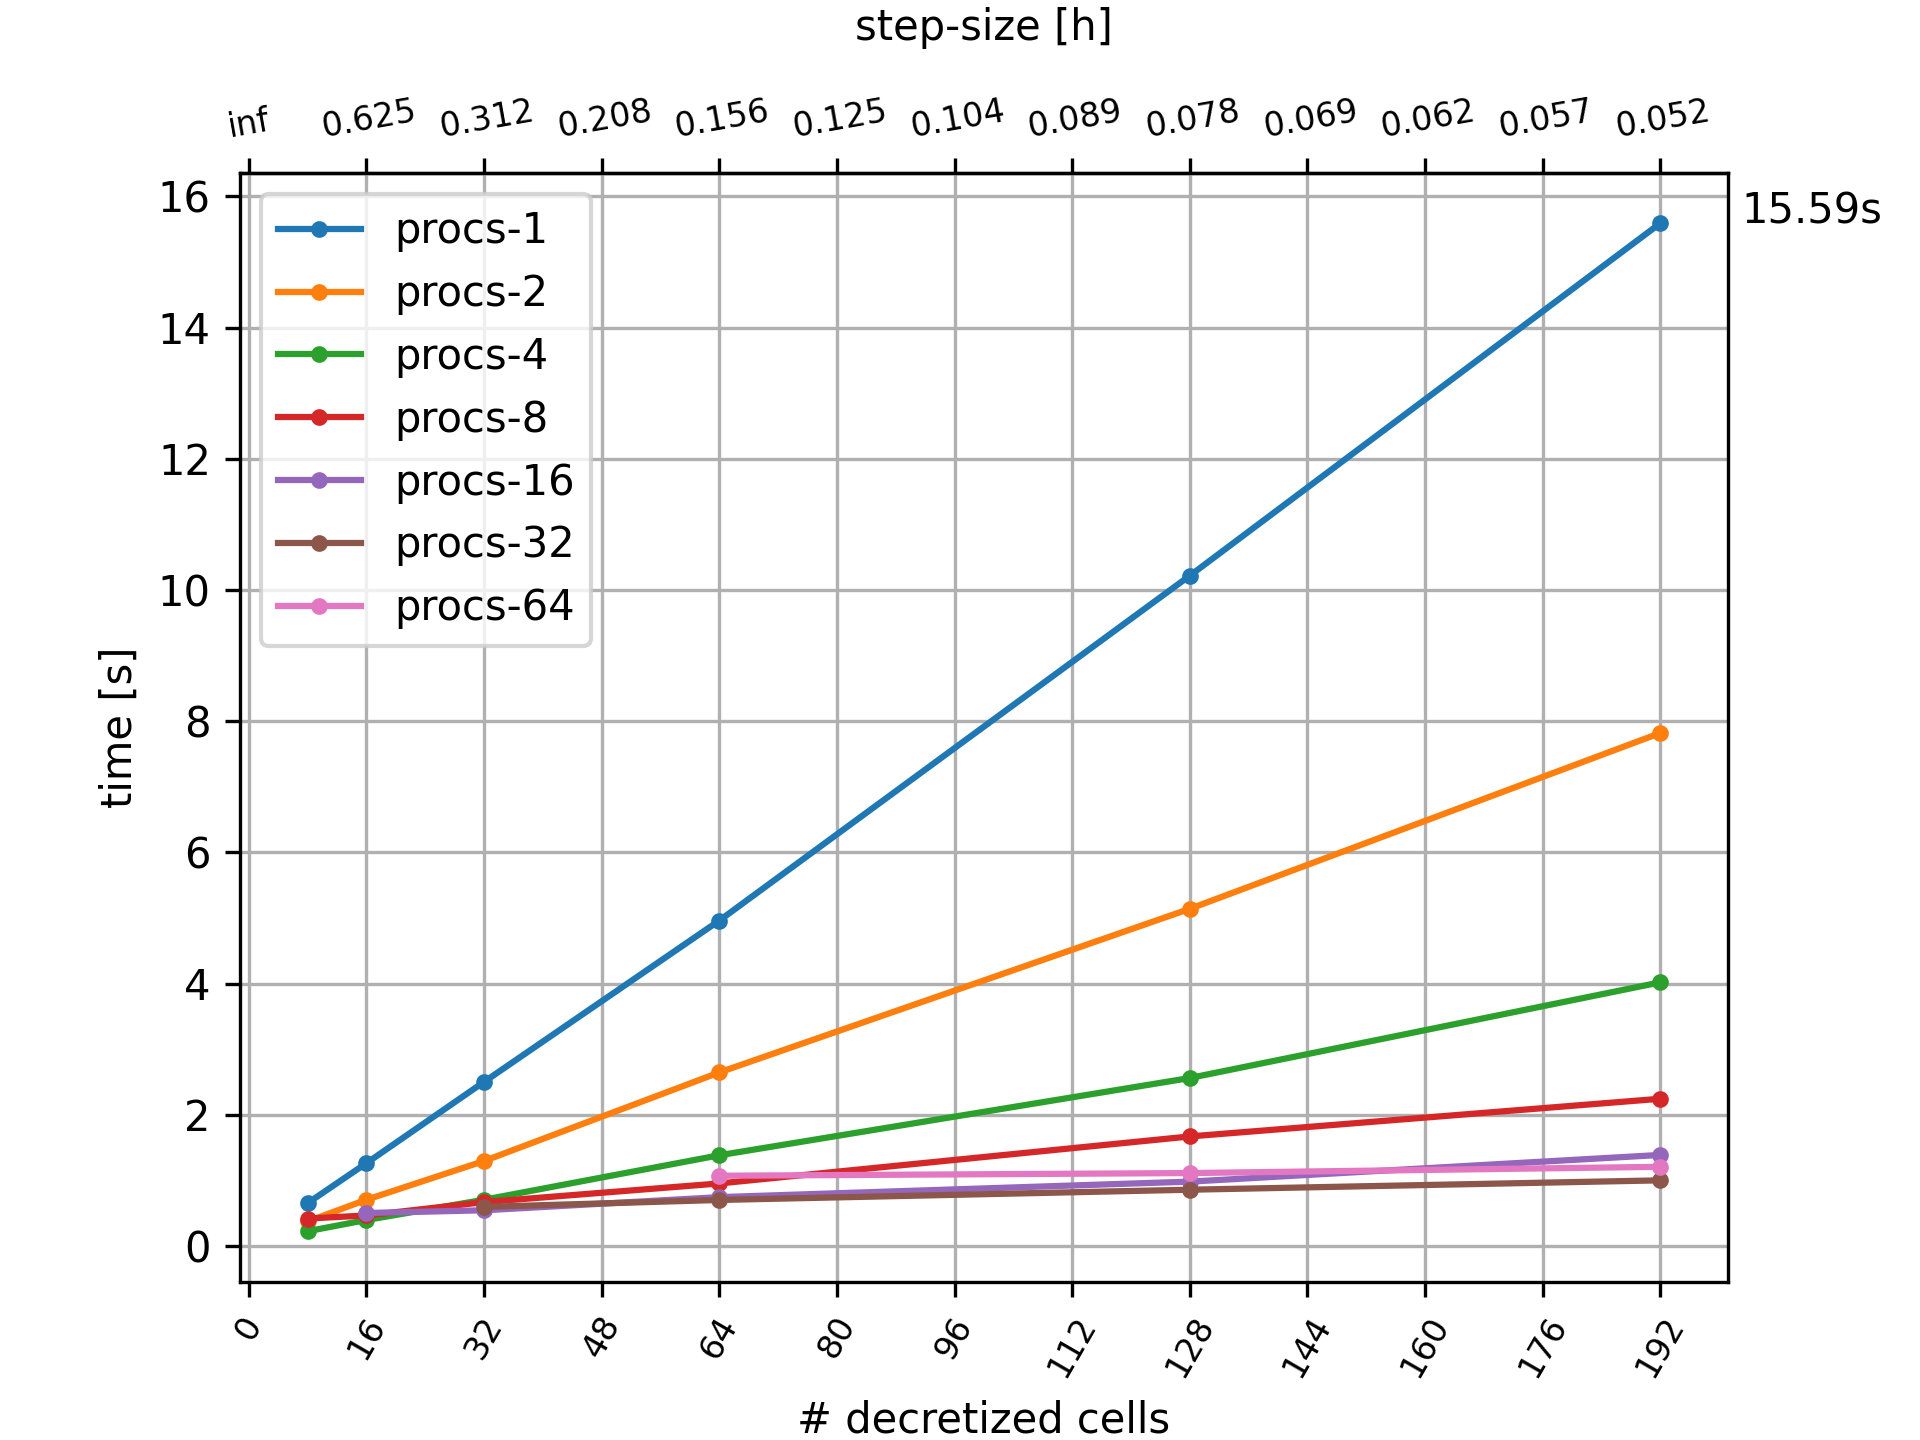
\includegraphics[width=0.7\textwidth]{figures/t301_const_proc_plot.png}
    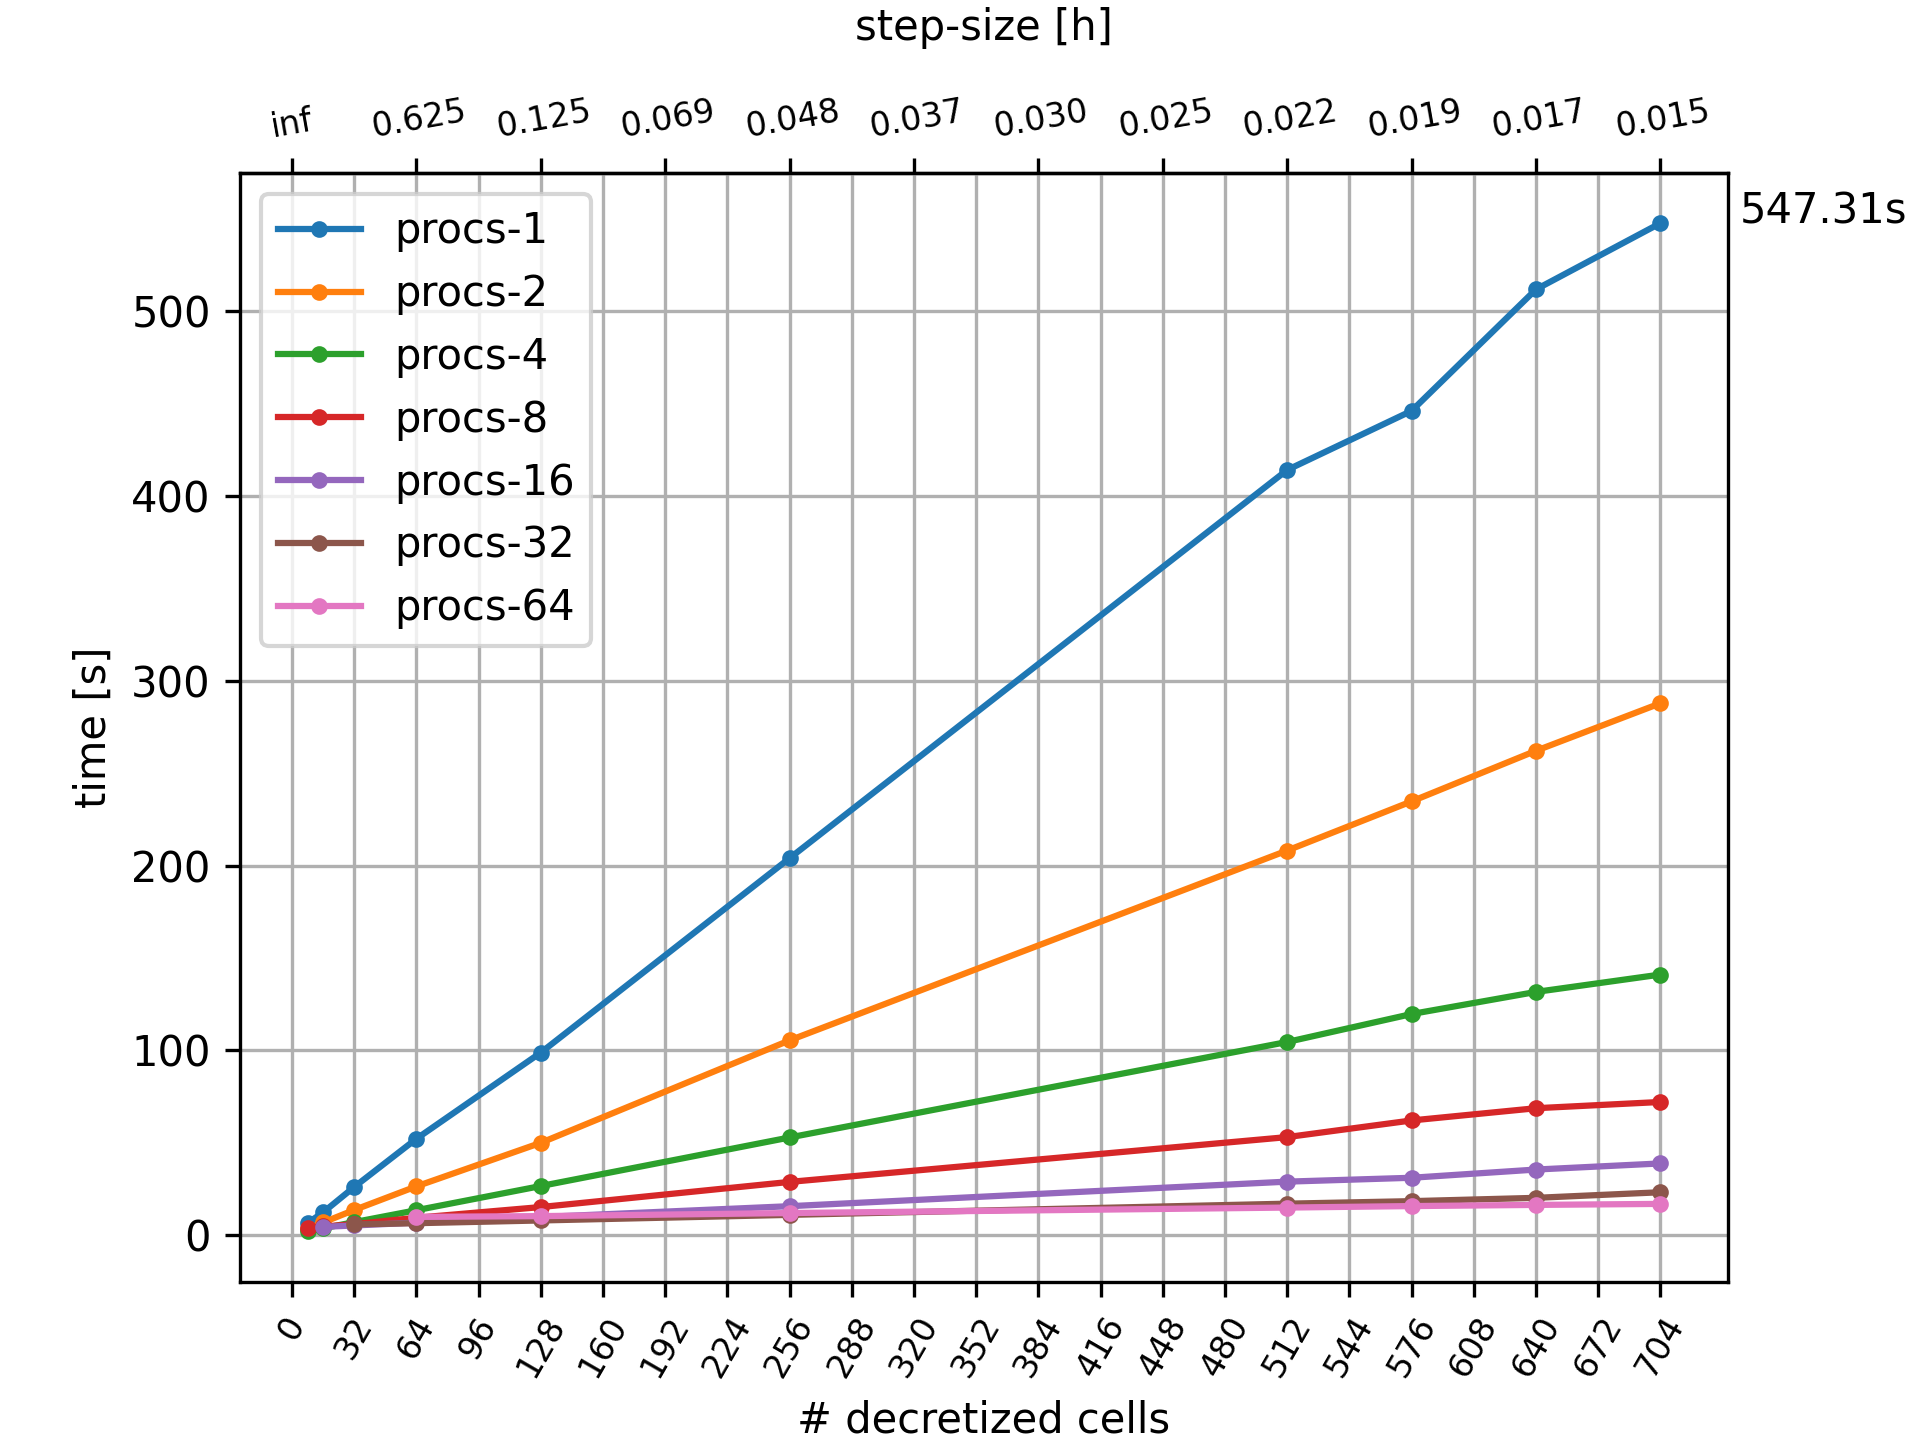
\includegraphics[width=0.7\textwidth, trim = 0 0 0 0.5cm, clip]{figures/t401_const_proc_plot.png}
    \caption{Execution times of all cases in \autoref{tab:DomainDecomposition1} (top) and \autoref{tab:DomainDecomposition2} (bottom)}
    \label{fig:allexec}
\end{figure}

It can be observed from \autoref{fig:allexec} that the doubling of speed-up with increase in processors (or the halving of execution times) is true for other problem sizes as well. We can also recognize the effect of communication overhead for \texttt{procs-64} in the plot at the top.
\pagebreak
\section{Conclusion}
The assumptions made in the implementation of the overall project is discussed in this section and the ideas for improvement are also briefly presented.

\subsection{Uneven Distrbution: \texttt{Scatterv()}}
The minimum step-size $h$ used in the serial method is not used in the parallel method, reason being that we wanted even distribution of the decomposed domain and also to always keep the number of processes as a power of 2. This is a voluntary choice to easily distribute the decomposition through a simple method \texttt{Scatter()}. However, if further customization is needed, we can make the distribution uneven as well using \texttt{Scatterv()}, for this the first \texttt{rank} will the remainder of the decomposed domain. The uneven distribution allows us to use any number of processes, with no issues in using the same minimum step-size as in the serial method.

\subsection{Final Thoughts}
The overall project was exciting as well as very informative. We, however, find using MPI in C/C++ a bit more clear and explicit as opposed to \texttt{mpi4py} in Python which we found a bit less intuitive and abstract. But this hands-on approach to an MPI Project really made us appreciate the usefulness of parallelization in research projects as well as numerical methods.
\newpage
\listoffigures
\listoftables


\newpage
\printbibliography
\end{document}
